\section{Methodology} 

\subsection{Metrics}
We compare our architecture incorporating \dio{} to a reinforcement learning architecture. 
Precisely for our scenario, we judge \emph{optimality}, i.e. the number of steps to reach the goal and 
\emph{safety}, i.e. ratio of successes to failures. Those metrics are analyzed during both training and deployment. 
We gather the cumulative rewards and cumulative rewards as well as the total number of failures and success over 180k frames of training, and 100 episodes of deployment. 

\subsection{Settings} 
Our above metrics and gathered for 8 different settings. We consider both $\alpha$, 0 (equivalent to rl alone), 0.5, 1, 3 and 9. 
Similarly, we consider two settings for the number of obstacles: (1)
minimal (5\% of the board is covered by obstacles), and (2)
intermediate (10\%).
For each, we gather the metrics described above. 

\subsection{Gathered Results} 

\paragraph{During Training.} For optimization purposes, training is done using multiprocessing reinforcement learning as indicated in figure~\ref{fig:multiprocess}. 
The network is loaded and parallel environments are spawned given the available number of processes. For $n$ frames, the rl routine is returned before the final experience is collected 
and used to update the parameters of the neural network. For our purpose, the cumulative reward is the reward of each $(obs_i, r_i)$ added over the number of updates. 
Similarly, the terminal states are computed according to this similar philosophy, meaning that at every given environment, if the resulting state is terminal and a failure, we add it to the cumulative failures to assess 
safety overtime. At the end of training, we compute the ratio of successes over failures to analyze the needed number of failures before convergence.

\begin{figure}[H]
    \centering
    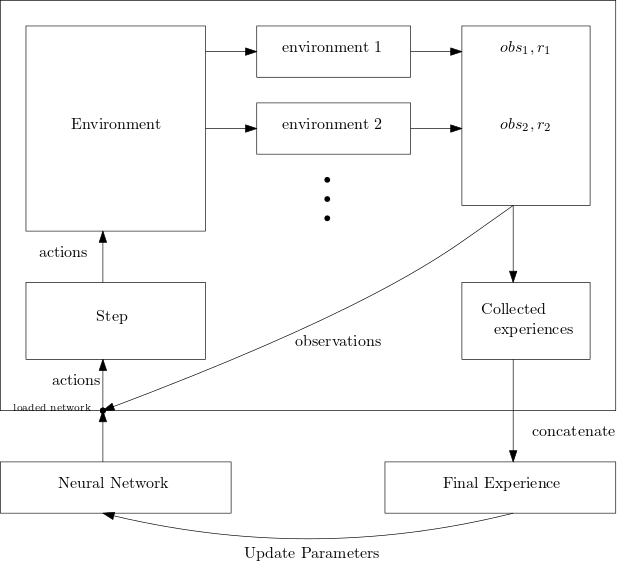
\includegraphics[scale=0.4]{figures/multiprocess.png}
    \caption{Multi-processing Reinforcement Learning}
    \label{fig:multiprocess}
  \end{figure}

  \paragraph{During Deployment.} Once training converges and a resulting policy is computed, we deploy the given policy for a 1000 episodes, given an episode ends either 
  with a success or a failure. We compute the average number of steps it takes to reach the goal and its standard deviation to assess the optimality of the resulting paths. 
  For safety, we still consider the ratio of success over failures as an indication. 
  
